% !TeX encoding = UTF-8
% !TeX spellcheck = it_IT
% !TeX root = MatDiz.tex

\documentclass[openany,10pt,italian]{dictionaryCD}
\errorcontextlines=9 
%\usepackage{refcheck}
\usepackage{lettrine}
\usepackage{rotating}
\usepackage{tabularx}

%======New command===============
%Simbolo per gradi Farenheit
\newcommand\gradiF{\ensuremath{\,^\circ F}}%Scrittura gradi Farenheit
%Istruzione \see riscritta: pochissimo usata 
\newcommand\vedi{\textit{vedi}}
%frazione in linea
\newcommand*\smallfrac[2]{\ensuremath{\mathop{{}^{#1}\!/\!_{#2}}\nolimits}}
%======Per SIunits===============
%\makeatletter
%\DeclareRobustCommand{\unit}[1]{\@inunitcommandtrue\ensuremath{\SI@fstyle{\@qsk\period@active{#1}}}}
%================================
\renewrobustcmd{\textlatin}[1]{\leavevmode{\latintext#1}}
\makeatletter
\def\@Roman#1{\expandafter\@slowromancap\romannumeral#1@}
%================================



%===============================
\includeonly{
A,
B,
C,
D,
E,
F,
G,
H,
I,
J,
K,
L,
M,
N,
O,
P,
Q,
R,
S,
T,
U,
V,
W,
X,
Y,
Z,
}
\input{../Mod_base/simboli_operatori}
\makeindex[title={\HUGE Indice dei nomi}]
\usepackage[autostyle,italian=guillemets]{csquotes}
%\usepackage[language=italian,backend=biber]{biblatex}
\usepackage[language=italian,style=philosophy-modern,backend=biber,sorting=ynt,hyperref,bibencoding=utf8,]{biblatex}

\addbibresource{MatDiz.bib}
\usepackage{standalone}
\standaloneconfig{mode=buildnew}
\listfiles
%\newcommand{\PrintMathFonts}{%
%	\count255=0
%	\loop\ifnum\count255<16
%	(\the\count255:~\fontname\textfont\count255)
%	\advance\count255 by 1
%	\repeat}
\newcolumntype{L}{>{\sffamily $}l<{$}}
% Geophysics
\DeclareSIUnit\gon{gon}
\DeclareSIUnit\cgon{cgon}
\DeclareSIUnit\mgon{mgon}
\usepackage{floatrow}
 \begin{document}
%	\PrintMathFonts
\hypersetup{pageanchor=false}
\setlength{\abovesectionskip}{4.0pt plus 0.5ex}
\setlength{\belowsectionskip}{-\belowsectionskip}
%------------------------------------------------
\lccode`\'=`\' % qualche file di lingua reimposta questo valore in modo globale a zero bisogna quindi restituirgli un valore diverso da zero!
\onecolumn
\pagecolor{StrongGray}
\thispagestyle{empty}
{\HUGE\bfseries Dizionario di Matematica}

$e^{-i\pi}=-1$
\vspace{30mm}
%==========================
{\topskip=0.1 in
\vfill

{\hfill{\textsf{\huge{\textbf{Claudio Duchi - 2017} }}}}

%\end{minipage}}%
\newpage%\pagecolor{white}\cleardoublepage[empty]
\pagecolor{white}
\pagestyle{empty}
\begin{center}
{\Large\textsc{CLAUDIO DUCHI - dizionario di MATEMATICA}}\\
\textcolor{rossovivo}{\vrule height 0.8pt width 160mm}\\[\baselineskip]
\end{center}

{\topskip=.2 in
\begin{minipage}{155mm}%
\vspace{80mm}
\begin{center}
{\Huge\bfseries Dizionario}\\[8pt]%
{\Huge\bfseries Glossario di Matematica}\\[8pt]%
\end{center}
\end{minipage}}%
\vfill
\begingroup
\begin{center}
\textcolor{rossovivo}{\vrule height 0.8pt width 160mm}
\end{center}
%\footnotesize
%%\setlength{\parindent}{0pt}
%%\setlength{\parskip}{\baselineskip}
%\textsc{PERMESSI DI DISTRIBUZIONE} - \textcopyright\ \& \textcopyleft\ Heinrich F. Fleck - MMXIII\,-\,MMXVI;  Versione 0.07\,-\,A-Z  \\
%Opera non commerciale liberamente a disposizione    secondo le specifiche di protezione totale nelle modalità garantite dalla licenza Creative Commons per le formule \textit{all rights~reserved} e \textit{no rights reserved}),  \textsf{\textsc{cc by-nc-nd}}: \textit{creativecommons.it}.\\
%Chiunque abbia in disponibilità questo lavoro potrà diffonderlo con ogni mezzo idoneo, purché conservi inalterati i testi e le specifiche connesse, ma è vietata la trasposizione su siti terzi dell'intera opera o di singole parti di essa: s'intendono soltanto autorizzate citazioni  con riferimento bibliografico; è ammesso da parte di terzi siti web il link  del file PDF al sito dell'autore.%Le traduzioni dei testi, quando non diversamente indicato, sono dell'autore.
%\\[3pt]
%\textit{www.heinrichfleck.net/marineria/marineria.html}\,\,-\,\,\textit{heinrich.fleck@yahoo.it}\hfill 
%\endgroup


\newpage 
%\newpage\textcolor{white}{  A  }
\thispagestyle{empty}

%\begin{figure}[t!]
%\centering\includegraphics[width=0.999\linewidth]{vespucci-taranto} \\[6pt]
%\end{figure}
%\vfill
%\begin{flushleft}
%\textcolor{sufred}{\rule{162mm}{0.3mm}\hspace{2mm}}\\
%In copertina, il Vespucci fotografato dal (quasi) gemello  Colombo nella metà degli anni trenta; qui sopra, il Vespucci invelato, con vento a 30 nodi, abbandona il mar Piccolo di Taranto  al comando dell'ammiraglio Agostino Straulino\index{Straulino Agostino} (1965); in quarta di copertina ancora il Vespucci ed il Colombo assieme  all'ancora  (1935); \textit{Archivio Storico Marina Militare Italiana}
%%\end{flushleft}

\frontmatter\pagenumbering{Roman}  %Modificato Claudio 14-01-2014
 
	\hypersetup{pageanchor=true}
%===============
\mainmatter 
\tableofcontents
\makeatletter
  \def\@Roman#1{\expandafter\textlatin\expandafter{%
                \expandafter\@slowromancap\romannumeral#1@}}
\csname @openrightfalse\endcsname
%===============

\twocolumn
\makeatletter
   \typeout{===========================================}
   \typeout{Larghezza di colonna pari a \the\columnwidth}
    \dimen@=0.35145980351\columnwidth
   \typeout{Larghezza di colonna pari a \strip@pt\dimen@\space mm}
   \typeout{===========================================}
\makeatother

% !TeX encoding = UTF-8
% !TeX spellcheck = it_IT
% !TeX root = MatDiz.tex
\chapter{A}
\vspace{5mm}
\lemma{adiacente}Attaccato, contiguo \pointsto~\seeentry{s. adiacente}
\entry{addendo}Termine dell'addizione\pointsto~\seeentry{addizione}.
\entry{addizione}Operazione che associa a una coppia di numeri, gli addendi, un numero detto somma\pointsto~\seeentry{somma}.
\lemma{Ahmes} Scriba egiziano che intorno al 1600 a.C trascrisse un papiro risalente a circa tre secoli prima. Tale papiro, noto come papiro di \pointsto~\seeentry{Papiro di Rhind}, è una delle fonti sulla matematica egizia.\index{Ahmes}
\lemma{algebra} Dall'arabo al-jabr \llemma{algebra booleana}\pointsto~\seeentry{Bool George}\index{Bool George} 
\lemma{algoritmo}Metodo o processo di calcolo che con regole fisse permette la soluzione di qualsiasi problema.
\lemma{algebrico}In matematica è un aggettivo che ha vari significati legate al contesto in cui si usa.
\llemma{a. equazione} Equazione che si ottiene ponendo uguale a zero un polinomio\pointsto~\seeentry{polinomio} $P(x)=0$.\llemma{a. numero}è una radice\pointsto~\seeentry{radice} di una equazione algebrica $P(x)=0$ i cui coefficienti sono tutti numeri razionali.
\lemma{Aleph-zero}Primo numero transfinito\pointsto~\vedilemma{n. transfinito}, rappresenta la cardinalità dei numeri naturali $\aleph_{0}$.
\lemma{al-Khwarizmi Muhammad ibn Musa}\index{al-Khwarizmi Muhammad ibn Musa}(780 circa 850) Persiano, matematico, astronomo, astrologo, geometra, nel 820 si trasferì a Baghdad dove fu chiamato a dirigerne la Biblioteca. Scrisse \textit{Al-jabr wa al-muqābala} che fu tradotto da Roberto di Chester\pointsto~\seeentry{Chester Roberto di} nel 1145. In pratica questo libro diede un nome a una materia l'algebra (al-jabr). Scrisse anche libro di cui rimane solo la traduzione latina \textit{Algoritmi de numero Indorum} dove introduce la numerazione indiana con le cifre moderne. Dalla latinizzazione del suo cognome nasce il termine algoritmo\pointsto~\seeentry{algoritmo} \cite{Gheverghese2000}\cite{Kline1972}.
\lemma{altezza}In un triangolo\pointsto~\seeentry{triangolo} è la perpendicolare\pointsto~\seeentry{perpendicolare} ad un segmento che passa per il vertice opposto\pointsto~\seeentry{o. vertice} al lato.
\lemma{analisi matematica}Branca della matematica che si è sviluppata a partire del seicento tramite i lavori di Leibniz\pointsto~\vedilemma{Leibniz Gottfried Wilhelm} e Newton\pointsto~\vedilemma{Newton Isaac}. Con l'introduzione del concetto di derivata\pointsto~\vedilemma{derivata} e d'integrale\pointsto~\vedilemma{integrale} è diventata uno strumento indispensabile per la ricerca moderna. 
\entry{AND}Operazione logica. La tabella di verità associata è~\vref{tab:AfunzioneAND}
\begin{table}
	\scaptionb{Funzione AND}
	\label{tab:AfunzioneAND}
	\centering
	\begin{tabular}{ccc}
	\toprule
	$A$&$B$&$AB$\\
	\midrule  
	0&0&0\\
	1&0&0\\
	0&1&0\\
	1&1&1\\
	\bottomrule
\end{tabular}
\end{table}
\begin{figure}%[!tb]
	\def\FrameCommand{\fboxsep=\FrameSep \colorbox{shadecolor}}% da def\FrameCommand{\fboxsep=\FrameSep\colorbox{shadecolor}}% da "shaded"
	\begin{MakeFramed}{\advance\hsize-\width \FrameRestore}% da "framed"
		\begin{center}%
			\textcolor{StrongGray}{\textsf{Da sessa-decimale a sessagesimale}}%
			\par%
			\vspace*{-\smallskipamount}%
			\vrule height 0.8pt width 56mm%
		\end{center}%
		\begin{small}%
			Supponiamo di avere un angolo $\alpha=35.2789^{\circ}$ e di volerlo convertire in sessagesimale. Procediamo come segue
			\begin{align*}
			35.2789^{\circ}=&35^{\circ}+0.2789^{\circ}\\
			0.2789^{\circ}=&(0.2789\cdot 60)^{'}=16.734^{'}\\
			16.734^{'}=&16^{'}+0.734^{'}\\
			0.734^{'}=&(0.734\cdot 60 )^{''}=44.04^{''}\\
			44.04^{''}=&44^{''}+0.04^{''}\\
			\ang{35.2789}=&\ang{35;16;44}
			\end{align*}
			La conversione è ultimata.
		\end{small}%
		\vspace*{-\smallskipamount}%
	\end{MakeFramed}%
\end{figure}%
\lemma{anello}Un insieme non vuoto R è un \textit{anello associativo} se in R sono definite due operazioni denominate $+$ e $\cdot$ rispettivamente, tali che per $a,b,c\in\; \R$
\begin{compactenum}
	\item $a+b\in R$
	\item $a+b=b+a$
	\item $(a+b)+c=a+(b+c)$
	\item $\exists\; 0\in R\;\text{tale che}\; a+0=a\;\forall a\in R$
	\item $\exists\; -a\in R\;\text{tale che}\; a+(-a)=0$
	\item $a\cdot b\in R$
	\item $(a\cdot b)\cdot c=a\cdot(b\cot c)$
	\item $a\cdot(b+c)=a\cdot b+a\cdot c$ e $(a+b)\cdot c=a\cdot c+b\cdot c$
\end{compactenum}
Le richieste da uno a cinque indicano che R è un gruppo abeliano\pointsto~\vedilemma{g. abeliano} rispetto a $+$. Gli ultimi assiomi indicano che R è chiuso rispetto ad un'operazione associativa\pointsto~\vedilemma{associativa}. \cite{Herstein1989}
\entry{angolo}Parte di piano compresa fra due semirette\pointsto~\seeentry{semiretta} che hanno la stessa origine. Le semirette sono chiamati lati, l'origine comune vertice. Si usano le lettere latine minuscole per indicare i lati, le lettere latine maiuscole per indicare i vertici e infine le lettere greche per indicare gli angoli.\llemma{a. concavo}Un angolo è concavo se contiene il prolungamento dei propri lati.\llemma{a. convesso}Un angolo è convesso se non è concavo.\llemma{a. giro}Un angolo è giro se è il doppio di un angolo piatto.
\llemma{a. nullo}Un angolo è nullo se i lati dell'angolo coincidono.\llemma{a. orientato}Dopo aver fissato un ordine tra i lati dell'angolo, un angolo è positivo se per andare dal primo lato al secondo si ruota in senso antiorario. Un angolo è negativo se si ruota in senso orario.\llemma{a. misura}Vi sono tre unità di misura: i gradi sessagesimali con la variante sessa-decimale, i gradi centesimali e i radianti.
\begin{minitoc}
	\mttitle{Gradi sessagesimali}
	\mtssubtitle{Gradi sessa-decimali}
	\mttitle{Gradi centesimali}
	\mttitle{Radianti}
\end{minitoc}
\mttitle{Gradi sessagesimali}Di origine babilonese,
un grado sessagesimale è definito come la trecentosessantesima parte di un angolo giro. Ammette come sottomultipli il minuto, uguale alla sessantesima parte di un grado e il secondo, pari alla sessantesima parte di un minuto.
\begin{align*}
\ang{1}=&\dfrac{angolo giro}{360}\\
\ang{;1;}=&\dfrac{\ang{1}}{60}\\
\ang{;;1}=&\dfrac{\ang{;1;}}{60}=\dfrac{\ang{1}}{3600}
\end{align*}
Un angolo viene indicato con $\alpha=x^\circ y'z''$
\mtssubtitle{Gradi sessa-decimali}
Nella versione sessa-decimale non si ha 
la suddivisione fra gradi, minuti e secondi ma l'ampiezza è indicata da un numero decimale. Angoli notevoli: un angolo retto misura \ang{90;;}, un angolo piatto \ang{180;;}.
\begin{figure}%[!tb]
	\def\FrameCommand{\fboxsep=\FrameSep \colorbox{shadecolor}}% da def\FrameCommand{\fboxsep=\FrameSep\colorbox{shadecolor}}% da "shaded"
	\begin{MakeFramed}{\advance\hsize-\width \FrameRestore}% da "framed"
		\begin{center}%
			\textcolor{StrongGray}{\textsf{Equivalenze }}%
			\par%
			\vspace*{-\smallskipamount}%
			\vrule height 0.8pt width 56mm%
		\end{center}%
		\begin{small}%
			\begin{align*}
			\SI{1}{\degree}=&\SI{1.111}{\gon}\\
			\SI{1}{\degree}=&\SI{0.0175}{\radian}\\
			\SI{1}{\radian}=&\SI{57.2958}{\degree}\\
			\SI{1}{\radian}=&\SI{63.662}{\gon}\\
			\SI{1}{\gon}=&\SI{1.111}{\degree}\\
			\SI{1}{\gon}=&\SI{0.0157}{\radian}
			\end{align*}
		\end{small}%
		\vspace*{-\smallskipamount}%
	\end{MakeFramed}%
\end{figure}%
\mttitle{Gradi centesimali}
Il grado centesimale (gon) è pari alla quattrocentesima parte di un angolo giro.
\begin{align*}
\SI{1}{\gon}=&\dfrac{angolo giro}{400}\\
\SI{1}{\cgon}=&\SI{1}{\per\gon\tothe{2}}\\
\SI{1}{\mgon}=&\SI{1}{\per\gon\tothe{3}}
\end{align*}
%\SI{1}{\gon}=\SI[parse-numbers = false]{\left(\frac{10}{9}\right)}{\degree}
Angoli notevoli: l'angolo retto misura \SI{100}{\gon}, angolo giro\SI{400}{\gon}
\mttitle{Radianti} Unità di misura dell'ampiezza dell'angolo piano che fa parte del SI\pointsto~\vedilemma{SI}. Simbolo rad. Un angolo ha ampiezza un radiante se presa una qualunque circonferenza, la lunghezza dell'arco intercettato è uguale al raggio. Un angolo giro è \SI{2\pi}{\radian}.
\llemma{a. piatto}Un angolo è piatto se i lati appartengono alla stessa retta.\llemma{a. retto}Un angolo è retto se uguale alla metà di uno piatto.
\lemma{anomalia}In un sistema di riferimento polare è l'angolo che il raggio vettore forma con l'asse di riferimento.
\lemma{appartenenza}Relazione che indica che un elemento appartiene ad un insieme. Simbolo $\in$
\lemma {apotema}Raggio della circonferenza inscritta\pointsto~\vedilemma{c. iscritta} in un poligono\pointsto~\vedilemma{poligono} regolare.
\lemma{arco}Parte di curve delimitata da due punti.
\lemma{arcoseno} Inversa della funzione coseno\pointsto~\vedilemma{coseno} è definita $\funzione{\arccos}{[-1,1]}{[0,\pi]}$. 
\lemma{arcseno}Inversa della funzione seno\pointsto~\vedilemma{seno} è definita $\funzione{\arcsin}{[-1,1]}{[-\frac{\pi}{2},\frac{\pi}{2}]}$. 
\lemma{arcotangente}Inversa della funzione tangente\pointsto~\vedilemma{tangente} è definita $\funzione{\arctan}{\R}{(-\frac{\pi}{2},\frac{\pi}{2})}$.\lemma{ascissa}
\entry{asintoto}L'asintoto è una retta che si avvicina indefinitamente a una curva. 
\llemma{a. verticale}La funzione\pointsto~\seeentry{funzione}$\funzione{f}{A}{B}$ ha un asintoto verticale per $a\in A$ se
$
\lim_{x\to a^+}f(x)=\pm\infty
$
oppure
$
\lim_{x\to a^-}f(x)=\pm\infty
$
\llemma{a. orizzontale}La retta $y=c$ è un asintoto orizzontale per la funzione $\funzione{f}{A}{B}$ se $
\lim_{x\to\pm\infty}f(x)=c
$	
\llemma{a. obliquo}La retta $y=mx+q$ è un asintoto obliquo per la funzione $\funzione{f}{A}{B}$ se
$
\lim_{x\to +\infty}[f(x)-(mx+q)]=0
$
o analogamente
$
\lim_{x\to -\infty}[f(x)-(mx+q)]=0
$
\lemma{associativa}Un'operazione binaria è associativa se 
$
(a*b)*c=a*(b*c)
$
\begin{figure}%[!tb]
	\def\FrameCommand{\fboxsep=\FrameSep \colorbox{shadecolor}}% da def\FrameCommand{\fboxsep=\FrameSep\colorbox{shadecolor}}% da "shaded"
	\begin{MakeFramed}{\advance\hsize-\width \FrameRestore}% da "framed"
		\begin{center}%
			\textcolor{StrongGray}{\textsf{Da sessagesimale a sessa-decimale}}%
			\par%
			\vspace*{-\smallskipamount}%
			\vrule height 0.8pt width 56mm%
		\end{center}%
		\begin{small}%
		Supponiamo di avere un angolo di $\alpha=\ang{25;40;20}$ e di volerlo convertire in sessa-decimale. Procediamo come segue
		\begin{align*}
		\alpha=&25^{\circ}+\left(\dfrac{40}{60}\right)^{\circ}+\left(\dfrac{20}{3600}\right)^{\circ}\\
		=&25^{\circ}+\left(\dfrac{2400+20}{3600}\right)^{\circ}\\
		=&25^{\circ}+\left(\dfrac{121}{180}\right)^{\circ}\\
		\approx&25^{\circ}+0.6722^{\circ}\\
		\approx&25.6722^{\circ}
		\end{align*}
		La conversione è ultimata.
		\end{small}%
		\vspace*{-\smallskipamount}%
	\end{MakeFramed}%
\end{figure}%


% !TeX encoding = UTF-8
% !TeX spellcheck = it_IT
% !TeX root = MatDiz.tex
\chapter{B}
\vspace{5mm} 
\lemma{baricentro}Punto in cui può essere concentrato tutto il peso di un corpo.\llemma{b. triangolo}In un triangolo punto d'incontro delle mediane\pointsto~\seeentry{mediana}.
\lemma{base}\titolettoa{In un sistema di numerazione}, numero di cifre, compreso lo zero, che servono ad rappresentare un numero.\titolettoa{Base potenza} nelle potenze, rappresenta il numero che deve essere moltiplicato per se stesso tante volte che è indicato dall'indice.\titolettoa{Base logarimo} Numero che ha per esponente il logaritmo\pointsto~\vedilemma{logaritmo} in modo da ottenere l'argomento.
\begin{figure}
	\centering
	\scaptionb{George Boole 1815-1864}
	\label{fig:georgeboolecolor}\floatfoot{Source: Di Haks-\url{http://www.enezeus.com/blog/wp-content/uploads/2006/10/hacker1.jpg}, Pubblico dominio,\url{https://commons.wikimedia.org/w/index.php?curid=1597609}}
	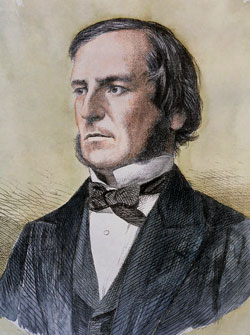
\includegraphics[width=0.7\linewidth]{Figure/B/George_Boole_color}
\end{figure}
\lemma{Bernoulli Daniel}\index{Bernoulli Daniel}(1700-1782) Nato a Groninga in Olanda il 29 gennaio 1700. Era figlio di Johann Bernoulli, nipote di Jacob Bernoulli, fratello più giovane di Nicolaus II Bernoulli, fratello più anziano di Johann II Bernoulli. Ha avuto pessimi rapporti con il padre anche lui matematico. Grande amico di Eulero\pointsto~\seeentry{Euler Leonard}\cite{Kline1972}
\begin{figure}
	\centering\scaptionb{Bernoulli Daniel 1700-1782}
	\label{fig:339px-eth-bib-bernoullidaniel1700-1782-portrait-portr10971}
	\floatfoot{By Unbekannt - E-Pics Bildarchiv online \url{http://doi.org/10.3932/ethz-a-000046381} \selectlanguage{english}{This image is from the collection of the ETH-Bibliothek and has been published on Wikimedia Commons as part of a cooperation with Wikimedia CH. Corrections and additional information are welcome. Public Domain,} \url{https://commons.wikimedia.org/w/index.php?curid=59419205}}
	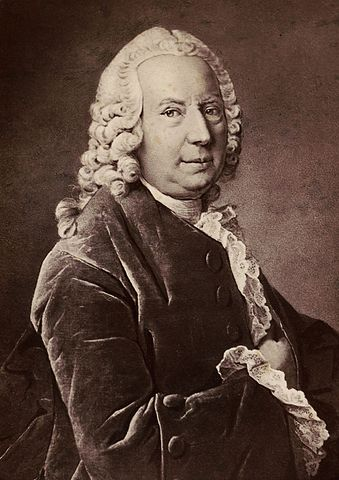
\includegraphics[width=0.7\linewidth]{Figure/B/Bernoulli_Daniel}
\end{figure}
\lemma{Bernoulli Jakob}(1654-1705) Fratello maggiore di Johann Bernoulli e zio di Daniel Bernoulli. Contribui allo sviluppo del calcolo infinitesimale. Tenne una corrispondenza con Gottfried Wilhelm von Leibniz\pointsto~\seeentry{Leibniz Gottfried Wilhelm}, uno dei fondatori del calcolo. La sua opera principale \textit{Ars Conjectandi}, pubblicata postuma nel 1713, contiene i fondamenti del calcolo delle probabilità.\index{Bernoulli Jakob}
\begin{figure}
\centering\scaptionb{Jakob Bernoulli (1654-1705)}
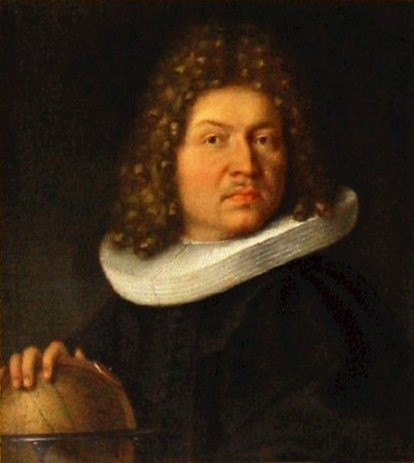
\includegraphics[width=0.7\linewidth]{Figure/B/Jakob_Bernoulli}
		\label{fig:jakobbernoulli}
\end{figure}
\lemma{Bernoulli Johann}\cite{Kline1972}\index{Bernoulli Johann}(1667-1748) Fratello di Jakob, fu allievo come lui di Leibniz\pointsto~\seeentry{Leibniz Gottfried Wilhelm}. contribui allo sviluppo del calcolo infinitesimale. Ebbe come allievo Eulero\pointsto~\seeentry{Euler Leonard}. Ebbe una controversia con Guillaume de l'Hopital  \pointsto~\vedilemma[Hopital Guillaume marchese de l']{Hôpital Guillaume marchese de l'}\ per l'omonima regola delle forme indeterminate.\index{Euler Leonard}
\begin{figure}
	\centering
\scaptionb{Johann I Bernoulli (1667-1748)}
	\label{fig:johannbernoulli}
	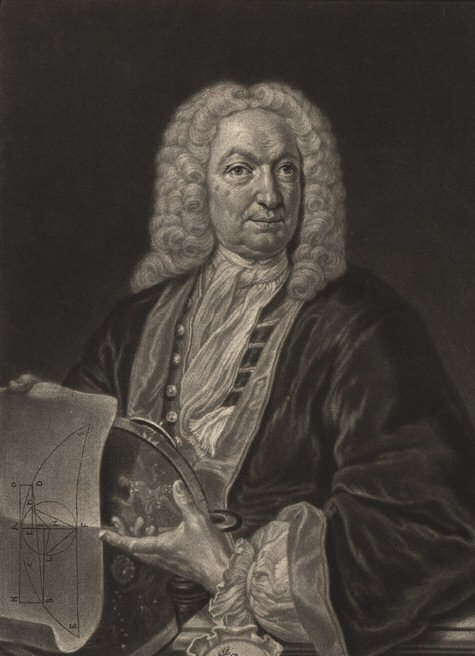
\includegraphics[width=0.7\linewidth]{Figure/B/Johann_Bernoulli}
\floatfoot{Di Johann Jakob Haid - Pubblico dominio, \url{https://commons.wikimedia.org/w/index.php?curid=57070}}
\end{figure}
\lemma{Bernoulli Nikolaus I}(1687-1759) Uno dei più importanti membri della famiglia Bernoulli. Era nipote di Jakob e Johann Bernoulli. Lavorò sulle equazioni differenziali e sulla geometria.
 \index{Bernoulli Nikolaus I}
 \lemma{Bernoulli Nikolaus II}(1695-1726) Fratello di Daniel Bernoulli. Contemporaneo di Eulero\pointsto~\seeentry{Euler Leonard} si trasferì a San Pietroburgo dove morì nel 1726. Successivamente la sua cattedra fu assegnata ad Eulero. 
 \cite{Kline1972}\index{Bernoulli Nikolaus II}
 \begin{figure}
 	\centering	\scaptionb{Nicolaus II Bernoulli (1695-1726)}
 	\label{fig:bernoullinicolausii}
 	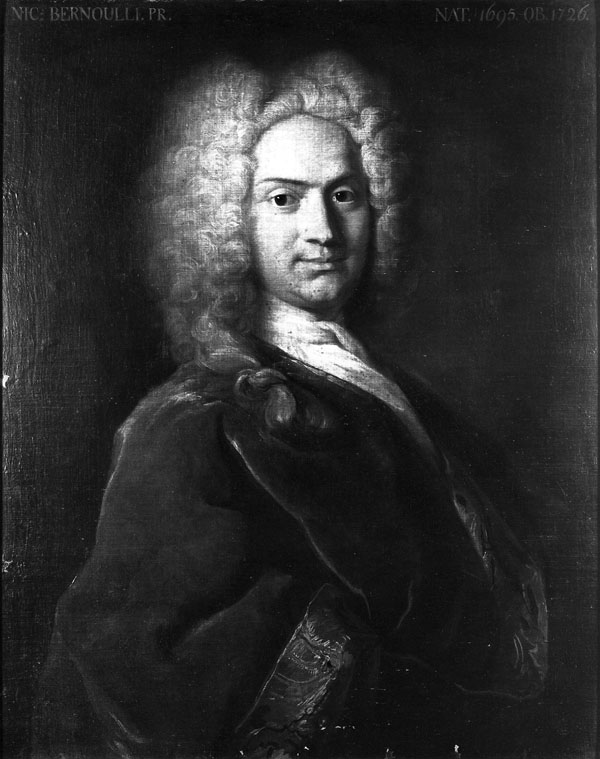
\includegraphics[width=0.7\linewidth]{Figure/B/Bernoulli_Nicolaussecondo}
 	\floatfoot{Di Johann Rudolf Huber - \url{http://www.simout.com/nicolaus-copernicus&page=327 } \url{https://commons.wikimedia.org/w/index.php?curid=10963524}}
  \end{figure}
\lemma{binario sistema}Sistema numerico a base due che usa le cifre \num{0} e \num{1} per rappresentare un numero.
\lemma{bisettrice}In un angolo\pointsto~\vedilemma{angolo}, semiretta\pointsto~\vedilemma{semiretta} con origine nel vertice, che divide l'angolo\pointsto~\vedilemma{angolo} in due parti uguali.
\lemma[Bolyai Janos]{Bolyai János}(1802-1860) Il suo contributo maggiore fu il suo lavoro nelle geometrie non euclidee.\index{Bolyai János}
\begin{figure}
	\centering
	\scaptionb[Janos Bolyai(1802 1860)]{János Bolyai(1802 1860)}
	\label{fig:bolyaijanosmarkosferencfestmenye}
	\floatfoot{Source: By Ferenc Márkos - Transferred from hu.wikipedia to Commons by Tambo., CC BY-SA 3.0, \url{https://commons.wikimedia.org/w/index.php?curid=24338736}}
	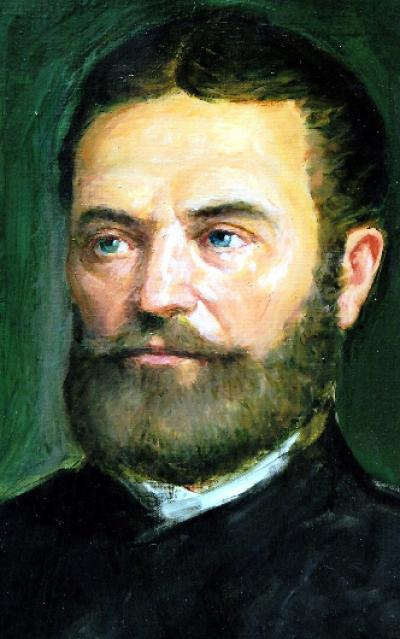
\includegraphics[width=0.7\linewidth]{Figure/B/Bolyai_Janos}
\end{figure}
\lemma{Bombelli Raffaele}\index{Bombelli Raffaele}(1526- ? 1572ca) Matematico e ingegnere diede una definizione chiara dei numeri negativi. Prese in considerazione i complessi nella risoluzione delle equazioni cubiche. Definì in termini moderni le quattro operazioni con i numeri complessi\vedilemma{n. complesso} anche se, non li accettava completamente (\textit{Algebra} 1572) \cite{Kline1972}.
\lemma{Bool George} (1815-1864)\index{Bool George}  nato a Lincoln il due novembre 1815 da un'umile famiglia. Nel 1854 pubblicò <<\textit{Indagine sulle leggi del pensiero}>>. Questo libro è alla base dell'algebra booleana. Il 24 novembre 1864 muore a Cork.\cite{Nahin2015} 
\lemma{Briggs Henry}(1561-1630)Scrisse la prima tabella dei logaritmi in base dieci \cite{Kline1972} nel 1617. Nel 1624  pubblicò \textit{Arithmetica logarithmica} ampliando tale tabella \cite{Boyer1980}.
\lemma{byte} Otto bit.
% !TeX encoding = UTF-8
% !TeX spellcheck = it_IT
% !TeX root = MatDiz.tex
\chapter{C} 
\vspace{5mm} 
\lemma{c} \titolettoa{simbolo} del grado centesimale.\titolettoa{simbolo} del capitale in matematica finanziaria.\titolettoa{simbolo} del cento nella numerazione latina.
\lemma{calcolo} Insieme di procedimenti atti a dare la soluzione di un dato problema matematico.\llemma{c. combinatorio}Parte della matematica che ha per scopo di contare i raggruppamenti di oggetti\pointsto~\vedilemma{permutazione}.
\lemma{campo}
\lemma{Cantor Georg} (1845 – 1918)\index{Cantor Georg}Fondatore della teoria degli insiemi introdusse il concetto di numero transfinito. 
\begin{figure}
	\centering
	\scaptionb{Georg Cantor (1845 – 1918)}
	\label{fig:georgcantor2}
	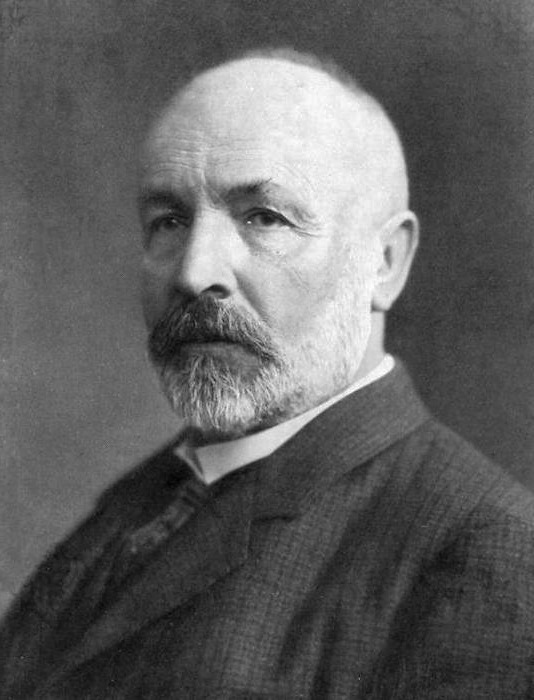
\includegraphics[width=0.7\linewidth]{Figure/C/Georg_Cantor2}
\end{figure}
\lemma{Cardano Gerolamo}(1501-1576)\index{Cardano Gerolamo}
\lemma{Cavalieri Bonaventura}(1598 1647)
\begin{figure}
	\centering
	\includegraphics[width=0.7\linewidth]{Figure/C/Jerôme_Cardan}
	\scaptionb{Girolamo Cardano (1501-1576)}
	\label{fig:jeromecardan}
\end{figure}
\begin{figure}
	\centering
	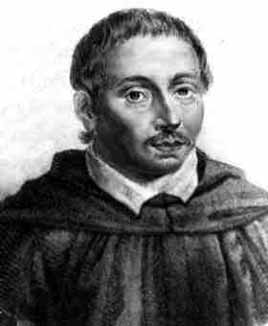
\includegraphics[width=0.7\linewidth]{Figure/C/Bonaventura_Cavalieri}
	\scaptionb{Cardano Gerolamo (1501-1576)}
	\label{fig:bonaventuracavalieri}
\end{figure}
\lemma{cateto} Lato di triangolo rettangolo\pointsto~\vedilemma{t. rettangolo} non opposto all'angolo retto\pointsto~\vedilemma{a. retto}.
\lemma{centro} Punto equidistante da tutti i punti della circonferenza.\llemma{c. delle masse} \pointsto~\vedilemma{baricentro} \cite{UTET1969} 
\llemma{c. di gravità} \'{E} il punto nel quale si può pensare applicata la forza peso del corpo.
\lemma{cicloide} Linea piana generata dal moto di un punto connesso rigidamente ad un cerchio che rotola senza strisciare.
\lemma{Chester Roberto di} \index{Chester Roberto di} Traduttore e arabista inglese lavorò intono al 1150. A lui si deve la prima traduzione parziale de libro \textit{al-Kitāb al-mukhtasar fī hisāb al-jabr wa al-muqābala} di al-Khwarizmi\pointsto~\vedilemma{al-Khwarizmi Muhammad ibn Musa} che tradusse in latino come \textit{Liber algebrae et almucabala} \cite{Gheverghese2000} 
\lemma{circonferenza} Luogo geometrico\pointsto~\vedilemma{luogo geometrico} dei punti del piano equidistanti da un punto fisso detto centro.\llemma{c. goniometrica} In un sistema di riferimento cartesiano\pointsto~\vedilemma{s. di riferimento cartesiano} è una circonferenza con centro nell'origine degli assi e raggio\pointsto~\vedilemma{raggio} unitario.\llemma{c. lunghezza} La lunghezza di una circonferenza di raggio $r$ è $l=2\pi r$.
\llemma{c. iscritta} 
\lemma{corda} Segmento\pointsto~\vedilemma{segmento} che congiunge due punti di una circonferenza\pointsto~\vedilemma{circonferenza} .
\lemma{coseno} Dato un triangolo rettangolo\pointsto~\vedilemma{t. rettangolo} definiamo coseno dell'angolo il rapporto tra il cateto\pointsto~\vedilemma{cateto} adiacente\pointsto~\vedilemma{s. adiacente} all'angolo e l'ipotenusa\pointsto~\vedilemma{ipotenusa} $\cos\beta=\frac{\text{adiacente} } {\text{ipotenusa} } $. Data una circonferenza goniometrica\pointsto~\vedilemma{c. goniometrica} diremo coseno l'ascissa\pointsto~\vedilemma{ascissa} del punto di intersezione tra il raggio\pointsto~\vedilemma{raggio} e la circonferenza \vref*{fig:cdefinizioneCoseno}.\llemma{c. funzione} 
\begin{figure} [b!]
	\scaptionb{Funzione coseno grafico} 
	\label{fig:cfunzioneCoseno} 
	\includestandalone[width=\linewidth]{Figure/cosenografico} 
\end{figure} 
La funzione coseno\pointsto~\vedilemma{goniometria} è definita in $\R$ a valore in $[-1,1]$. La funzione è limitata\pointsto~\vedilemma{f. limitata}.
La funzione è periodica\pointsto~\seeentry{f. periodica} di periodo $k\pi\quad k\in\Z$. La figura~\vref{fig:cfunzioneCoseno} rappresenta il grafico della funzione.
\lemma{coppia} Elemento dell'insieme prodotto cartesiano\pointsto~\vedilemma{p. cartesiano} $A\times B$. Si indica con $\left(a,b\right)\quad a\in A,\, b\in B$.\llemma{c. ordinata} Una coppia è ordinata se $\left(a,b\right)\neq\left(b,a\right)$. 
\lemma{crescente} \pointsto~\vedilemma{f. crescente} .
\begin{figure} 
	\scaptionb{Coseno definizione} 
	\label{fig:cdefinizioneCoseno} 
	\includestandalone[width=\linewidth]{Figure/cosenodefinizione} 
\end{figure} 
% !TeX encoding = UTF-8
% !TeX spellcheck = it_IT
% !TeX root = MatDiz.tex
\chapter{D}
\vspace{5mm} 
\lemma{derivata}
\lemma{diametro}Corda\pointsto~\vedilemma{corda} che passa per il centro\pointsto~\vedilemma{centro} di una circonferenza\pointsto~\vedilemma{circonferenza}.
\lemma{dominio}Data una funzione $\funzione{f}{A}{B}$ il dominio è l'insieme dei punti di $A$ dove $f$ è definita.
% !TeX encoding = UTF-8
% !TeX spellcheck = it_IT
% !TeX root = MatDiz.tex
\chapter{E}
\vspace{5mm} 
\lemma{e} Costante numerica. $e$ numero irrazionale \pointsto~\seeentry{n. irrazionale} trascendente \pointsto~\seeentry{n. trascendente}. Nel 1728 Euler lo usa come base dei logaritmi naturali.
\lemma{Euclide}\index{Euclide}
\lemma{Euler Leonard}\index{Euler Leonard}(1707-1783) Nato vicino a Basilea. Fu allievo di Johann I Bernulli\pointsto~\vedilemma{Bernoulli Johann}\index{Bernulli Johann} trasferitosi all'accademia di S.Pietroburgo li divenne assistente di Daniel Bernulli \pointsto~\vedilemma{Bernoulli Daniel}\index{Bernulli Daniel} per poi succedergli. La sua produzione è sterminata in tutti i campi della matematica ed oltre. Il 7 settembre 1783 secondo le parole del marchese di Condorcet, <<cesso di calcolare e di vivere>>. 
\begin{figure}
	\centering
	\scaptionb{Leonhard Euler (1707-1783)}
	\label{fig:leonhardeuler}
	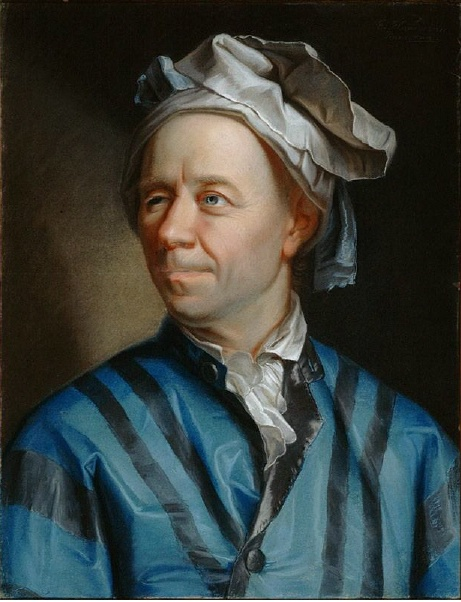
\includegraphics[width=0.7\linewidth]{Figure/E/Leonhard_Euler}
	\floatfoot{\selectlanguage{english}{Di Jakob Emanuel Handmann - 2. Kunstmuseum Basel1. digitized version, the source (scanner) of the digitized image is unknown.The image was transferred from en.wiki (en:Image:Leonhard Euler.jpg) under the {{PD-old}} license tag. Wars 16:56, 25 June 2006 (UTC), Pubblico dominio,} \url{https://commons.wikimedia.org/w/index.php?curid=893656}}
\end{figure}

% !TeX encoding = UTF-8
% !TeX spellcheck = it_IT
% !TeX root = MatDiz.tex
\chapter{F}
\vspace{5mm}
\lemma{fattoriale}
\lemma{figura}Ogni insieme di punti o linee o  superfici.\llemma{f. piana}Figura tutta contenuta in un piano.
\entry{funzione}
Una funzione è una relazione\pointsto~\seeentry{relazione} che ad ogni elemento di $x\in A$ dominio\pointsto~\seeentry{dominio}, fa corrispondere uno e uno solo elemento appartenente a $B$ codominio.
\begin{equation*}
\function{f}{A}{B}{x}{f(x)}
\end{equation*}
\llemma{f. algebrica}
Una funzione $\funzione{f}{A}{B}$ si dice algebrica\pointsto~\vedilemma{algebrico} se costruita utilizzando un numero finito di applicazioni delle quattro operazioni dell'aritmetica, dell'elevazione a potenza e delle radici.
\llemma{f. algebrica razionale}
Una funzione $\funzione{f}{A}{B}$ algebrica è razionale quando la variabile indipendente non si trova sotto il segno di radice.\llemma{f. algebrica irrazionale}Una funzione $\funzione{f}{A}{B}$ algebrica è irrazionale quando la variabile indipendente si trova sotto il segno di radice.
\llemma{f. algebrica intera}Una funzione $\funzione{f}{A}{B}$ algebrica è intera quando la variabile indipendente non si trova al denominatore di una frazione.\llemma{f. algebrica fratta} una funzione $\funzione{f}{A}{B}$ algebrica\pointsto~\vedilemma{algebrico} è fratta quando la variabile indipendente si trova al denominatore di una frazione.\llemma{f. trascendente}Una funzione $\funzione{f}{A}{B}$ è trascendente quando compaiono operazioni non algebriche come logaritmo, esponenziale, goniometriche.
\llemma{f. biettiva}Una funzione $\funzione{f}{A}{B}$ è biettiva se è contemporaneamente suriettiva e iniettiva.
\llemma{f. crescente}Una funzione $\funzione{f}{A}{B}$ è crescente in senso stretto nell'intervallo $I\subset A$ se
$\forall\; x_1,x_2\in I\quad x_1< x_2\Longrightarrow f(x_1)<f(x_2).$
%%%%%%%%
\llemma{f. dispari}Una funzione $\funzione{f}{A}{B}$ è una funzione dispari se $f(-x)=-f(x)\quad\forall x\in A$.\llemma{f. decrescente}Una funzione $\funzione{f}{A}{B}$ si dice decrescente in senso stretto nell'intervallo $I\subset A$ se
$\forall\; x_1,x_2\in I\quad x_1< x_2\Longrightarrow f(x_1)>f(x_2)$.\llemma{f. iniettiva}Una funzione $\funzione{f}{A}{B}$ è iniettiva se
$x_1\neq x_2\quad\Longrightarrow\quad f(x_1)\neq f(x_2)\quad \forall x_1,x_2\in A $ oppure $f(x_1)= f(x_2)\quad\Longrightarrow\quad x_1= x_2\quad \forall x_1,x_2\in A$.\llemma{f. non crescente}Una funzione $\funzione{f}{A}{B}$ si dice non crescente nell'intervallo $I\subset A$ se $\forall\; x_1,x_2\in I\quad x_1< x_2\Longrightarrow f(x_1)\geq f(x_2)$.\llemma{f. non decrescente}Una funzione $\funzione{f}{A}{B}$ si dice non decrescente nell'intervallo $I\subset A$ se $\forall\; x_1,x_2\in I\quad x_1< x_2\Longrightarrow f(x_1)\leq f(x_2)$. \llemma{f. limitata}Una funzione $\funzione{f}{A}{B}$ è una funzione limitata se $\exists\; M\quad \abs{f(x)}<M \quad\forall x\in A$.\llemma{f. periodica}\'{E} una funzione $\funzione{f}{A}{B}$ di periodo $T>0$ se $f(x+kT)=f(x)\quad k\in \Z$\llemma{f. pari} una funzione $\funzione{f}{A}{B}$ è una funzione pari se $f(-x)=f(x)\quad\forall x\in A$.\llemma{f. suriettiva}Una funzione $\funzione{f}{A}{B}$ è suriettiva se $f(A)=B$\llemma{f. zeri}\pointsto~\vedilemma{z. funzione}
\lemma{frazione}
\llemma{f. egizia} 
Una frazione è egizia quando viene scritta come somma di frazioni con numeratore unitario.\cite{Boyer1980}. Metodi di calcolo ed esempi sono stati trovati nel papiro di Rhind\pointsto~\vedilemma{Papiro di Rhind}.

% !TeX encoding = UTF-8
% !TeX spellcheck = it_IT
% !TeX root = MatDiz.tex
\chapter{G}
\vspace{5mm} 
\lemma{goniometria}
\lemma{grado}\llemma{g. sessagesimale}\pointsto~\vedilemma{a. misura}\llemma{g. sessa-decimale}\pointsto~\vedilemma{a. misura}\llemma{g. centesimali}\pointsto~\vedilemma{a. misura}
\lemma{gruppo}\llemma{g. abeliano}
% !TeX encoding = UTF-8
% !TeX spellcheck = it_IT
% !TeX root = MatDiz.tex
\chapter{H}
\vspace{5mm}
\lemma[Hopital Guillaume marchese de l']{Hôpital Guillaume marchese de l'}\index{Hôpital Guillaume marchese de l'}
\begin{figure}
	\centering\scaptionb{Guillaume François Antoine marchese de l'Hôpital (1661-1704)}
	\includegraphics[width=0.7\linewidth]{Figure/H/Guillaume_de_l'Hôpital}
	\label{fig:guillaumedelhopital}
\end{figure}
A lui di deve la pubblicazione del primo libro sul calcolo differenziale nel 1696 \textit{Analyse des infiniment petits pour l'intelligence des lignes courbes}

% !TeX encoding = UTF-8
% !TeX spellcheck = it_IT
% !TeX root = MatDiz.tex
\chapter{I}
\vspace{5mm} 
\lemma{incognita}Quantità non nota, non conosciuta. L'uso delle incognite venne introdotto dal matematico francese Fraçois Viète\pointsto~\seeentry[Viete Francois]{Viète François} nel 1571.\index{Viète Fraçois}
\lemma{insieme}Lista, collezione o classe di oggetti
che sia ben definita o per meglio dire univocamente definita. Per indicare un insieme si usano le lettere maiuscole. Per indicare un elemento si usano le lettere minuscole. Un insieme può essere definito per elencazione o tramite la proprietà che lo caratterizza.\cite{Lipschutz1980}
\lemma{intervallo}Sottoinisieme della retta reale compreso tra due estremi detti estremo sinistro e destro\pointsto~\vedilemma{segmento}.\llemma{i. illimitato superiormente} ha l'estremo destro è $+\infty$. \llemma{i. illimitato inferiormente} ha l'estremo sinistro è $-\infty$.\llemma{i. illimitato} ha per estremo sinistro $-\infty$ e per estremo destro $+\infty$.
\lemma{integrale}
\lemma{ipotenusa}Lato maggiore di un triangolo rettangolo\pointsto~\vedilemma{t. rettangolo}.


% !TeX encoding = UTF-8
% !TeX spellcheck = it_IT
% !TeX root = MatDiz.tex
\chapter{J}
\vspace{5mm}
\lemma{Jones William}(1675-1749)Fu il primo ad associare il simbolo $\pi$ al rapporto tra circonferenza e diametro\pointsto~\seeentry{pi greco}.\index{Jones William}
\begin{figure}
	\centering\scaptionb{William Jones (1675 - 1749)}
	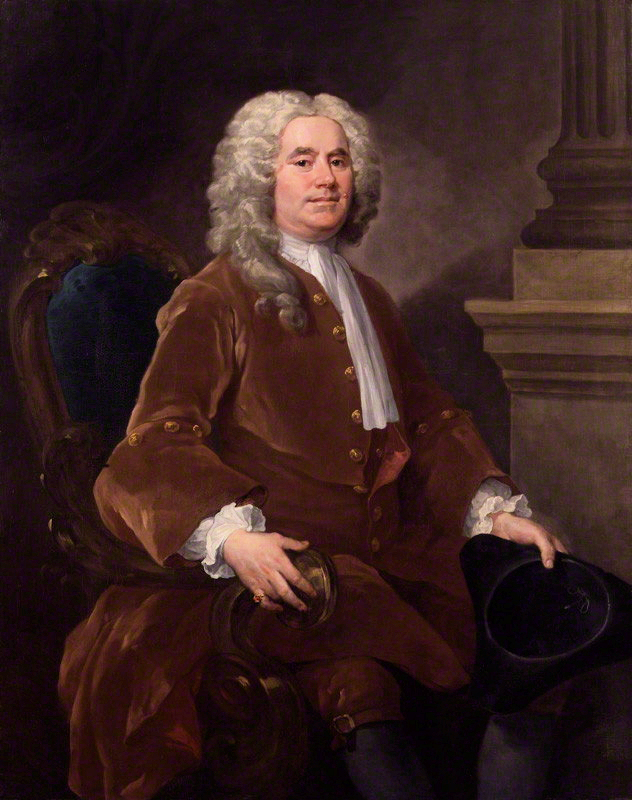
\includegraphics[width=0.7\linewidth]{Figure/J/William_Jones,_the_Mathematician}
		\label{fig:williamjonesthemathematician}
\end{figure}

% !TeX encoding = UTF-8
% !TeX spellcheck = it_IT
% !TeX root = MatDiz.tex
\chapter{K}
\vspace{5mm}
% !TeX encoding = UTF-8
% !TeX spellcheck = it_IT
% !TeX root = MatDiz.tex
\chapter{L}
\vspace{5mm} 
\lemma{lato}In geometria può indicare sia un segmento che una semiretta.\llemma{l. adiacente} ad un angolo. Un lato è adiacente ad un angolo se il lato coincide con un lato dell'angolo.\llemma{l. poligono}Segmento che congiunge due vertici consecutivi di un poligono.
\llemma{l. consecutivo}Due lati sono consecutivi se appartengono allo stesso poligono e sono segmenti consecutivi.\pointsto~\vedilemma{s. consecutivo}.\llemma{l. opposto} In un poligono due lati distinti e non consecutivi si dicono opposti.
Gottfried Wilhelm von Leibniz
\lemma{Leibniz Gottfried Wilhelm}\index{Leibniz Gottfried Wilhelm}
\lemma{logaritmo}Il logaritmo è l'esponente che bisogna dare alle base per ottenere l'argomento $x=\log_{a}b\,\Longleftrightarrow\,a^x=b\,a>0,\,a\neq1,\,b>0$. \llemma{l. funzione}Una funzione logaritmica è una funzione $\funzione{f}{\Rpos}{\R}$ di equazione $y=\log_{a}x$.\llemma{l. naturale} se la base è $e$\pointsto~\vedilemma{e} il logaritmo si dice naturale  e si scrive $\ln$
$\log_{e}b=\ln b$\llemma{l. decimale} se la base è dieci il ogaritmo è detto decimale o di \pointsto~\vedilemma{Briggs Henry} e si scrive $\log$
$\log_{10}b=\log b$
\lemma{luogo geometrico}Insieme di punti che godono tutti della stessa proprietà.
\begin{figure}
	\centering
	\scaptionb{Gottfried Wilhelm von Leibniz (1646-1716)}
	\label{fig:leibnizhannover}
	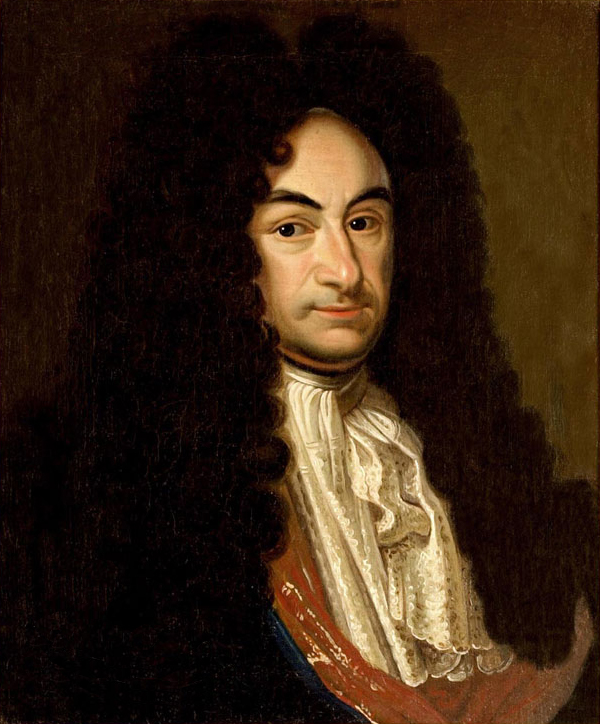
\includegraphics[width=0.7\linewidth]{Figure/L/Leibniz_Hannover}
\end{figure}

% !TeX encoding = UTF-8
% !TeX spellcheck = it_IT
% !TeX root = MatDiz.tex
\chapter{M}
\vspace{5mm}
\lemma{mediana} In un triangolo\pointsto~\vedilemma{triangolo} è il segmento che unisce il punto medio\pointsto~\vedilemma{p. medio} di un lato con il vertice opposto.
\lemma{multiplo}
\lemma{moltiplicazione}$ab=\dfrac{(a+b)^2-(a-b)^2}{4}$ \cite{Derbyshire2011}
% !TeX encoding = UTF-8
% !TeX spellcheck = it_IT
% !TeX root = MatDiz.tex
\chapter{N}
\vspace{5mm}
\lemma{NAND}Operazione logica. Tabella di verità associata è~\vref{tab:NfunzioneNAND}
\begin{table}
	\scaptiona{Funzione NAND}
	\label{tab:NfunzioneNAND}
	\centering
	\begin{tabular}{ccc}
		\toprule
	$A$&$B$&$A\mathbin{\overline{\wedge}}B$\\
	\midrule
	0&0&1\\
	1&0&1\\
	0&1&1\\
	1&1&0\\
	\bottomrule
	\end{tabular}
\end{table}
\lemma{Napier}\index{Napier} Definì i logaritmi inventandone il termine.
\lemma{Newton Isaac}\index{Newton Isaac}
\begin{figure}
	\centering
	\scaptionb{Isaac Newton (1642-1727)}
	\label{fig:godfreykneller-isaacnewton-1689}
	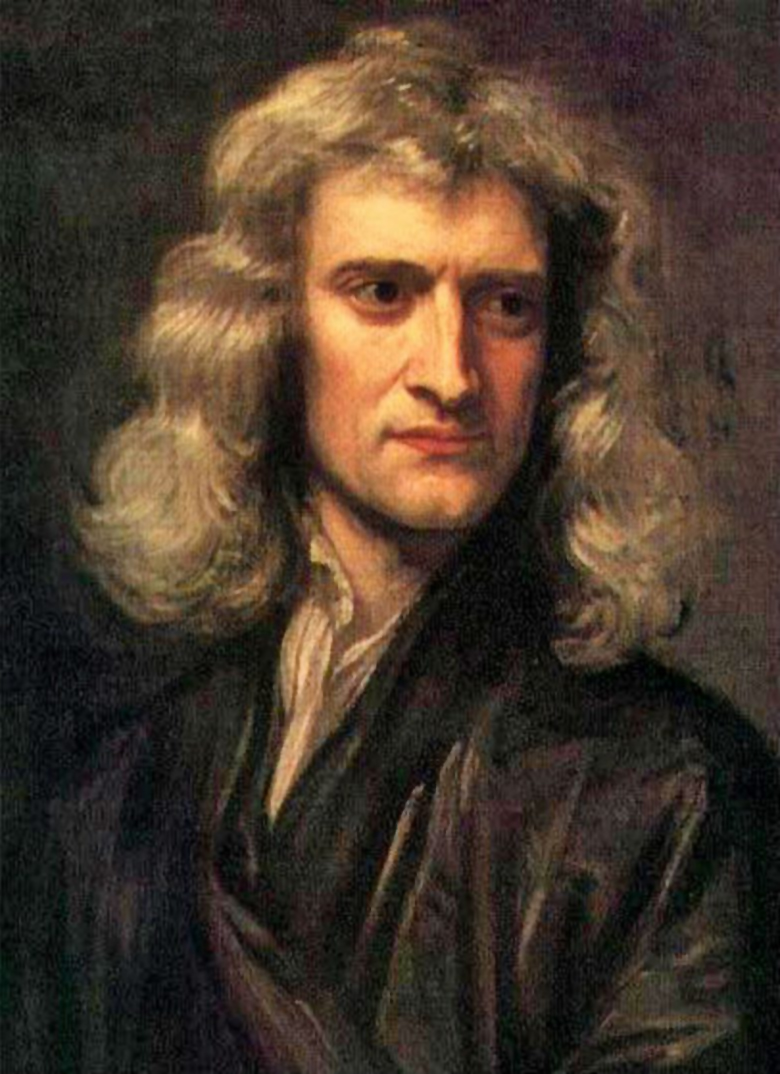
\includegraphics[width=0.7\linewidth]{Figure/N/GodfreyKneller-IsaacNewton-1689}
\end{figure}
\lemma{NOT}Operazione logica. Tabella di verità associata è~\vref{tab:NfunzioneNOT}
\begin{table}
	\centering
	\begin{tabular}{cc}%
		\toprule
		$A$&$\overline{A}$\\
		\midrule 
		1&0\\
		0&1\\
		\bottomrule
	\end{tabular}
	\scaptiona{Funzione NOT}
\label{tab:NfunzioneNOT}
\end{table}
\lemma{numero}
\llemma{n. complesso} \llemma{n. irrazionale}Un numero è irrazionale se non è possibile scriverlo come rapporto fra due numeri.\llemma{n. razionale} Un numero è razionale se può essere scritto come rapporto di due numeri interi. Il secondo numero deve essere diverso da zero $q=\frac{a}{b}\quad a,b\in \Z\; b\neq 0$. \llemma{n. trascendente}. \llemma{n. transfinito}
\begin{figure}%[!htb]
	\def\FrameCommand{\fboxsep=\FrameSep \colorbox{shadecolor}}% da def\FrameCommand{\fboxsep=\FrameSep\colorbox{shadecolor}}% da "shaded"
	\begin{MakeFramed}{\advance\hsize-\width \FrameRestore}%    da "framed"
		\begin{center}%
			\textcolor{StrongGray}{\textsf{$\sqrt{2}$ è irrazionale}}%
			\par%
			\vspace*{-\smallskipamount}%
			\vrule height 0.8pt width 56mm%
		\end{center}%
		\begin{small}%
			Supponiamo che $\sqrt{2}$ è un numero razionale. Se è razionale allora:
			\begin{align*}
		\sqrt{2}=&\dfrac{a}{b}
		\intertext{con $a$ e $b$ due numeri irriducibili.  Elevando al quadrato}
		2=&\dfrac{a^2}{b^2}\\
a^2=&2b^2
\intertext{quindi se $a^2$ è un multiplo di due $a$ è pari. Ma se $a$ è pari}
a=&2k\\
4k^2=&2b^2\\
b^2=&4k^2\\
\intertext{quindi se $b^2$ è un multiplo di due $b$ è pari}
			\end{align*}
Quindi abbiamo due numeri irriducibili che abbiamo dimostrato essere entrambi pari e quindi riducibili. Assurdo $\sqrt{2}$ non può essere razionale.			
		\end{small}%
		\vspace*{-\smallskipamount}%
	\end{MakeFramed}%
\end{figure}%
\lemma{numerabile}Un insieme è numerabile se può essere messo in corrispondenza con l'insieme dei numeri naturali.
% !TeX encoding = UTF-8
% !TeX spellcheck = it_IT
% !TeX root = MatDiz.tex
\chapter{O}
\vspace{5mm}
\lemma{OR}Operazione logica. La tabella di verità associata è~\vref{tab:OfunzioneOR}
\begin{table}
	\scaptiona{Funzione OR}
	\label{tab:OfunzioneOR}
	\centering
	\begin{tabular}{ccc}
	\toprule
$A$&$B$&$A+B$\\
\midrule         
0&0&0\\
1&0&1\\
0&1&1\\
1&1&1\\
\bottomrule
\end{tabular}
\end{table}
\lemma{ordinata}
\lemma{opposto}Ha significati sia geometrici che numerici.\llemma{o. angolo}Due angoli sono opposti se hanno il vertice in comune e i lati di uno sono  il prolugamento dell'altro.
\llemma{o. numero}In matematica dato un numero $a$ il suo opposto è quel numero che sommato ad $a$ da come somma\pointsto~\vedilemma{somma} zero\pointsto~\vedilemma{zero}.\llemma{o. vertice}Un vertice\pointsto~\vedilemma{vertice} è opposto ad un lato se non è uno dei suoi estremi.\llemma{o. lato} In un triangolo un lato\pointsto~\vedilemma{lato} è opposto ad un angolo\pointsto~\vedilemma{angolo} se non concorre a delimitarlo.
% !TeX encoding = UTF-8
% !TeX spellcheck = it_IT
% !TeX root = MatDiz.tex
\chapter{P}
\vspace{5mm}
\lemma{Papiro di Rhind}\pointsto~\seeentry{Rhind Henry} 
noto anche come papiro di Ahmes\pointsto~\seeentry{Ahmes}\index{Ahmes} uno scriba che lo  compilò nel 1650 a.C partendo da una fonte di tre secoli prima. Fu trovato a Luxor da Henry Rhind\index{Rhind Henry} che nel 1858 lo donò al 
\foreignlanguage{english}{British Museum}. Il papiro inizia con un elenco di frazioni nella forma $2/n$ che sono espresse come somma di frazioni egizie. Il papiro  contiene una raccolta di ottantasette  problemi. Viene considerato come una delle maggiori fonti della matematica egizia. \cite{Gheverghese2000}
\begin{figure}[!htb]
\def\FrameCommand{\fboxsep=\FrameSep \colorbox{shadecolor}}% da def\FrameCommand{\fboxsep=\FrameSep\colorbox{shadecolor}}% da "shaded"
\begin{MakeFramed}{\advance\hsize-\width \FrameRestore}%    da "framed"
\begin{center}%
\textcolor{StrongGray}{\textsf{Moltiplicazione egizia}}%
\par%
\vspace*{-\smallskipamount}%
\vrule height 0.8pt width 56mm%
\end{center}%
\begin{small}%
La moltiplicazione egizia si basa sulla duplicazione. Supponiamo che il nostro scriba volesse moltiplicare settanta per venticinque. Per prima  cosa doveva decidere chi stava per essere essere moltiplicato. 

Poniamo che venticinque moltiplichi settanta. Ahmes\index{Ahmes} avrebbe organizzato il lavoro in questo modo. Nella prima riga scriveva uno e settanta. La tabella è costruita in modo che ogni riga è il doppio della riga precedente. Questo procedimento di duplicazione termina quando il numero a sinistra supera, in questo caso, venticinque.%
\begin{center}
\begin{tabular}{LL}
\toprule 
1 & 70 \\ 
2 & 140 \\ 
4 & 280 \\ 
8 & 560 \\ 
16 & 1120 \\ 
\bottomrule
\end{tabular} 
\end{center}
Per prima cosa il nostro scriba avrebbe individua to nella colonna di sinistra i numeri la cui somma è uguale a 25 \[ 25=1+8+16\] Successivamente avrebbe sommato i corrispondenti numeri della seconda colonna ottenendo il prodotto. In notazione moderna\[ 70\times 25=70+560+1120=1750 \]Il procedimento si basa sul fatto che ogni numero può essere scritto come somma di potenze del  due \[25=1\cdot 2^0+0\cdot 2^2+1\cdot 2^3+1\cdot2^4  \] e successivamente l'uso della proprietà distributiva.
\end{small}%
\vspace*{-\smallskipamount}%
\end{MakeFramed}%
\end{figure}%
\lemma{parabola}Luogo geometrico dei punti del piano equidistanti da un punto fisso detto fuoco e da una retta fissa detta direttrice.
\lemma{parallele} Si dice di rette o piani che non hanno punti in comune. \llemma{p. postulato} Il quinto postulato\pointsto~\seeentry{postulato}  di Euclide\pointsto~\seeentry{Euclide} recita  \textit{Data una retta e un punto esterno ad esso per il punto passa una e una sola retta parallela alla retta data.}. 
\lemma{parallelepipedo} Poliedro a sei facce due a due parallele.
\lemma{parallelogramma} Quadrilatero con i lati opposti sono paralleli e uguali.
\lemma{parentesi} in un'espressione variano l'ordine con cui devono essere svolte delle operazioni. Vennero introdotte da {Viète\pointsto~\seeentry[Viete Francois]{Viète François} nel 1593 circa\cite{Kline1972}\index{Viète Fraçois}
\lemma{pari} Un numero è pari se è un multiplo\pointsto~\seeentry{multiplo} del due.
\lemma{Pascal Blaise} (1623-1662)\index{Pascal Blaise}
\begin{figure}
	\centering\scaptionb{Blaise Pascal (1623-1662)}
	\label{fig:pascalblaise}
	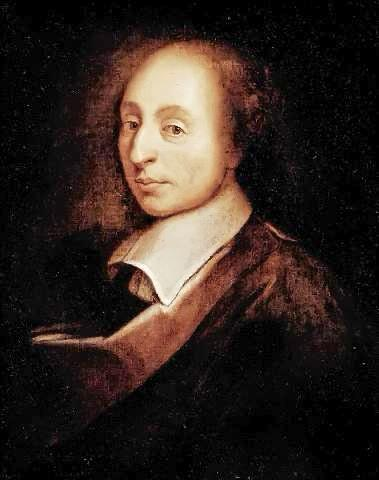
\includegraphics[width=0.7\linewidth]{Figure/P/Pascal_Blaise}
\end{figure}Ragazzo prodigio diede molti contributi alla matematica finché, dopo un esaurimento nervoso, di diede alla teologia. Fondamentali i suoi contributi al calcolo della probabilità. Introdusse il concetto di pressione. Nel 1642 costruì la sua prima macchina calcolatrice, la pascalina.
\lemma{Peano Giuseppe}  (1858-1932)\index{Peano Giuseppe}
\lemma{perimetro}Misura della lunghezza del contorno di una figura piana\pointsto~\seeentry{f. piana}. Viene indicato  con il simbolo $2P$.%
\lemma{permutazione}Dati n elementi distinti, tutti i possibili raggruppamenti formati da n oggetti, senza ripetizioni,  e che differiscano solo per l'ordine con cui sono formati si chiamano permutazioni semplici. Il simbolo è $P_n$, dove n indica il numero degli elementi. Il numero delle permutazioni è  $P_n=n!$.
\lemma{perpendicolare} Una retta è perpendicolare ad un'altra retta se ha un solo punto in comune con essa e forma quattro angoli retti.
\lemma{piano}Per Euclide\pointsto~\seeentry{Euclide}\index{Euclide} ente geometrico fondamentale insieme a punto e retta. \llemma{p. cartesiano}%
\begin{figure}[!htb]
	\def\FrameCommand{\fboxsep=\FrameSep \colorbox{shadecolor}}% da def\FrameCommand{\fboxsep=\FrameSep\colorbox{shadecolor}}% da "shaded"
	\begin{MakeFramed}{\advance\hsize-\width \FrameRestore}%    da "framed"
		\begin{center}%
\textcolor{StrongGray}{\textsf{Divisione egizia}}%
			\par%
			\vspace*{-\smallskipamount}%
			\vrule height 0.8pt width 56mm%
		\end{center}%
		\begin{small}%
		La divisione segue uno schema simile alla moltiplicazione. Poniamo di voler trovare il risultato di \[ 750\div 15\]
		\begin{center}
			\begin{tabular}{cc}
			\toprule
				1 & 15 \\ 
				2 & 30 \\ 
				4 & 60 \\ 
				8 & 120 \\ 
				16 & 240 \\ 
				32 & 480 \\ 
			\bottomrule
			\end{tabular} 
		\end{center}
	Nella colonna di destra individuo i numeri la cui somma è il dividendo\[750=480+240+30\] La somma dei corrispondenti numeri della colonna di sinistra da il quoziente\[ 50=2+16+32\]
		\end{small}%
		\vspace*{-\smallskipamount}%
	\end{MakeFramed}%
\end{figure}%
\lemma{Peirce Benjamin}(1809-1880)\index{Peirce Benjamin}
\lemma{pi greco}Numero irrazionale\pointsto~\seeentry{n. irrazionale} trascendente\pointsto~\seeentry{n. trascendente} corrispondente al rapporto tra una circonferenza\pointsto~\seeentry{circonferenza} e il suo  diametro\pointsto~\seeentry{diametro}. Il simbolo $\pi$ fu introdotto nel 1706 da  William Jones\pointsto~\seeentry{Jones William}.
%
%\begin{figure}[!htb]
%	\def\FrameCommand{\fboxsep=\FrameSep \colorbox{shadecolor}}% da def\FrameCommand{\fboxsep=\FrameSep\colorbox{shadecolor}}% da "shaded"
%	\begin{MakeFramed}{\advance\hsize-\width \FrameRestore}%    da "framed"
%		\begin{center}%
%			\textcolor{StrongGray}{\textsf{Pi greco}}%
%			\par%
%			\vspace*{-\smallskipamount}%
%			\vrule height 0.8pt width 56mm%
%		\end{center}%
%		\begin{small}%
%			Durante i secoli vi sono state varie rappresentazioni numeriche di $\pi$ 
%		\begin{center}
%			\begin{tabularx}{\linewidth}{XlX}
%	
%				1650 a.C. & Papiro di  Ahmes & $\pi\approx 3.16$\\ 
%			1600 a.C. & Tavoletta di Susa & $\pi\approx 3.125$\\ 
%			800 -- 500 a.C.	&Sulbasutra  &  $\pi\approx 3.09$\\ 
%			250 a.C. 	&Archimede  &   $\pi\approx\num{3.14}$\\ 
%			150 a.C. 	&Umasvati &   $\pi\approx\num{3.16}$\\ 
%			260 d.C. 	&Liu Hui  &   $\pi\approx\num{3.1416}$\\ 
%		480 d.C. 	&Tsu Chhung-Chih  &  $\num{3.1415926}<\pi<\num{3.1415927}$\\
%			500 d.C.	&Arybhata  & $\pi\approx\num{3.1416}$ \\ 
%			1400	&Madhava  & $\pi~\approx~\num{3.14159265359} $\\ 
%				&  &  \\ 
%				&  &  \\ 
%			\bottomrule
%			\end{tabularx} 
%		\end{center}
%		\end{small}%
%		\vspace*{-\smallskipamount}%
%	\end{MakeFramed}%
%\end{figure}%
\lemma{piramide} Poliedro costituito da una base poligonale e da altre formate da triangoli con il vertice in comune.
\lemma{Pitagora}\index{Pitagora}\llemma{P. teorema} In un triangolo rettangolo la somma dei quadrati costruiti su i cateti è equivalente al quadrato costruito sull'ipotenusa
\lemma{poliedro}figura solida delimitata da poligoni non complanari piani. Ogni lato è in comune a due di essi. Il punto di incontro di più lati è chiamato vertice.
\lemma{poligonale}Insieme ordinato di segmenti consecutivi non adiacenti.\llemma{p. aperta} Una poligonale è aperta se il primo estremo e l'ultimo non si intersecano. Una poligonale è aperta intrecciata se il primo estremo e l'ultimo non si intersecano ma i segmenti hanno almeno  un punto in comune.\llemma{p. chiusa} Una poligonale è chiusa se il primo estremo e l'ultimo estremo  si intersecano. Una poligonale è chiusa intrecciata se il primo estremo e l'ultimo  si intersecano e i segmenti hanno almeno  un punto in comune.
\lemma{poligono}Figura geometrica piana\pointsto~\seeentry{f. piana} limitata da tre o più segmenti\pointsto~\seeentry{segmento} che formino una poligonale chiusa non intrecciata\pointsto~\seeentry{p. chiusa}.
\lemma{polinomio}Somma di monomi non simili.
\lemma{postulato}
\lemma{prodotto} 
\lemma{punto}Per Euclide\pointsto~\seeentry{Euclide}\index{Euclide} ente geometrico fondamentale insieme a piano e retta.\llemma{p. medio}Punto equidistante dagli estremi di un segmento\pointsto~\vedilemma{segmento}.
\begin{table}[t]
\scaptionb{Tabella delle frazioni 2/n del papiro Rhind}\label{PapiroRhindtabella}%
\centering%
\begin{shadedtabular}[paglierino]{LL}
\toprule	
\frac{2}{3}=\frac{1}{2}+\frac{1}{6}&\frac{2}{5}=\frac{1}{3}+\frac{1}{15}\\
\frac{2}{7}=\frac{1}{4}+\frac{1}{28}&\frac{2}{9}=\frac{1}{6}+\frac{1}{18}\\
\frac{2}{11}=\frac{1}{6}+\frac{1}{66}&\frac{2}{13}=\frac{1}{8}+\frac{1}{52}+\frac{1}{104}\\

\frac{2}{15}=\frac{1}{10}+\frac{1}{30}&\frac{2}{17}=\frac{1}{12}+\frac{1}{51}+\frac{1}{68}\\
\frac{2}{19}=\frac{1}{12}+\frac{1}{76}+\frac{1}{114}&\frac{2}{21}=\frac{1}{14}+\frac{1}{42}\\
\frac{2}{23}=\frac{1}{12}+\frac{1}{276}&\frac{2}{25}=\frac{1}{15}+\frac{1}{75} \\

\frac{2}{27}=\frac{1}{18}+\frac{1}{54}&\frac{2}{29}=\frac{1}{24}+\frac{1}{58}+\frac{1}{174}+\frac{1}{232}\\
\frac{2}{31}=\frac{1}{20}+\frac{1}{124}+\frac{1}{155}&\frac{2}{33}=\frac{1}{22}+\frac{1}{66}\\
\frac{2}{35}=\frac{1}{30}+\frac{1}{42}&\frac{2}{37}=\frac{1}{24}+\frac{1}{111}+\frac{1}{296}\\

\frac{2}{39}=\frac{1}{26}+\frac{1}{78}&\frac{2}{41}=\frac{1}{24}+\frac{1}{246}+\frac{1}{328}\\
\frac{2}{43}=\frac{1}{42}+\frac{1}{86}+\frac{1}{129}+\frac{1}{301}&\frac{2}{45}=\frac{1}{30}+\frac{1}{90}\\
\frac{2}{47}=\frac{1}{30}+\frac{1}{141}+\frac{1}{470}&\frac{2}{49}=\frac{1}{28}+\frac{1}{196} \\

\frac{2}{51}=\frac{1}{34}+\frac{1}{102}&\frac{2}{53}=\frac{1}{30}+\frac{1}{318}+\frac{1}{795}\\
\frac{2}{55}=\frac{1}{30}+\frac{1}{330}&\frac{2}{57}=\frac{1}{38}+\frac{1}{114}\\
\frac{2}{59}=\frac{1}{36}+\frac{1}{236}+\frac{1}{531}&\frac{2}{61}=\frac{1}{40}+\frac{1}{244}+\frac{1}{488}+\frac{1}{610}\\ 

\frac{2}{263}=\frac{1}{42}+\frac{1}{126}&\frac{2}{65}=\frac{1}{39}+\frac{1}{195}\\
\frac{2}{67}=\frac{1}{40}+\frac{1}{335}+\frac{1}{536}&\frac{2}{69}=\frac{1}{46}+\frac{1}{138}\\
\frac{2}{71}=\frac{1}{40}+\frac{1}{568}+\frac{1}{710}&\frac{2}{73}=\frac{1}{60}+\frac{1}{219}+\frac{1}{292}+\frac{1}{365}\\

\frac{2}{75}=\frac{1}{50}+\frac{1}{150}&\frac{2}{77}=\frac{1}{44}+\frac{1}{308}\\
\frac{2}{79}=\frac{1}{60}+\frac{2}{237}+\frac{1}{316}+\frac{1}{790}&\frac{2}{81}=\frac{1}{54}+\frac{1}{162}\\
\frac{2}{83}=\frac{1}{60}+\frac{1}{332}+\frac{1}{415}+\frac{1}{498}&\frac{2}{85}=\frac{1}{51}+\frac{1}{255} \\

\frac{2}{87}=\frac{1}{58}+\frac{1}{174}&\frac{2}{89}=\frac{1}{60}+\frac{1}{356}+\frac{1}{534}+\frac{1}{890}\\
\frac{2}{89}=\frac{1}{70}+\frac{1}{130} &\frac{2}{93}=\frac{1}{62}+\frac{1}{186}\\
\frac{2}{95}=\frac{1}{60}+\frac{1}{380}+\frac{1}{570}&\frac{2}{97}=\frac{1}{56}+\frac{1}{679}+\frac{1}{776} \\ 

\frac{2}{99}=\frac{1}{66}+\frac{1}{198}&\frac{2}{101}=\frac{1}{101}+\frac{1}{202}+\frac{1}{303}+\frac{1}{606}\\
\bottomrule
\end{shadedtabular}%
\end{table}
% !TeX encoding = UTF-8
% !TeX spellcheck = it_IT
% !TeX root = MatDiz.tex
\chapter{Q}
\vspace{5mm}
% !TeX encoding =UTF-8
% !TeX spellcheck =it_IT
% !TeX root =MatDiz.tex
\chapter{R}
\vspace{5mm} 
\lemma{radice}
\lemma{radiante}\pointsto~\vedilemma{a. misura}
\lemma{reciproco}
\lemma{Recorde Robert} (1510-1558)\index{Recorde Robert} Scrisse il primo trattato inglese di algebra \foreignlanguage{english}{\textit{The Whetstone of Witte}}  dove venne usato per la prima volta il simbolo $=$ nel  1557\cite{Kline1972}.
\begin{figure}
\centering\scaptionb{Robert Recorde (1510-1558)}
	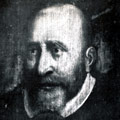
\includegraphics[width=0.7\linewidth]{Figure/R/Robert_recorde}
	\label{fig:robertrecorde}
\end{figure}
\lemma{Rhind Henry}Alexander Henry (1833–1863) Scozzese, archeologo trovò in un mercato di Luxor nel 1858, il papiro che porta il suo nome\index{Rhind Henry}. 
\lemma{raggio}Segmento che ha per estremi il centro di una circonferenza\pointsto~\vedilemma{circonferenza} e un punto di questa. 
\begin{figure}
	\centering\scaptionb{Alexander Henry Rhind (1833–1863)}
	\label{fig:frontispiecetomemoirofthelatealexanderhenryrhindofsibster}
	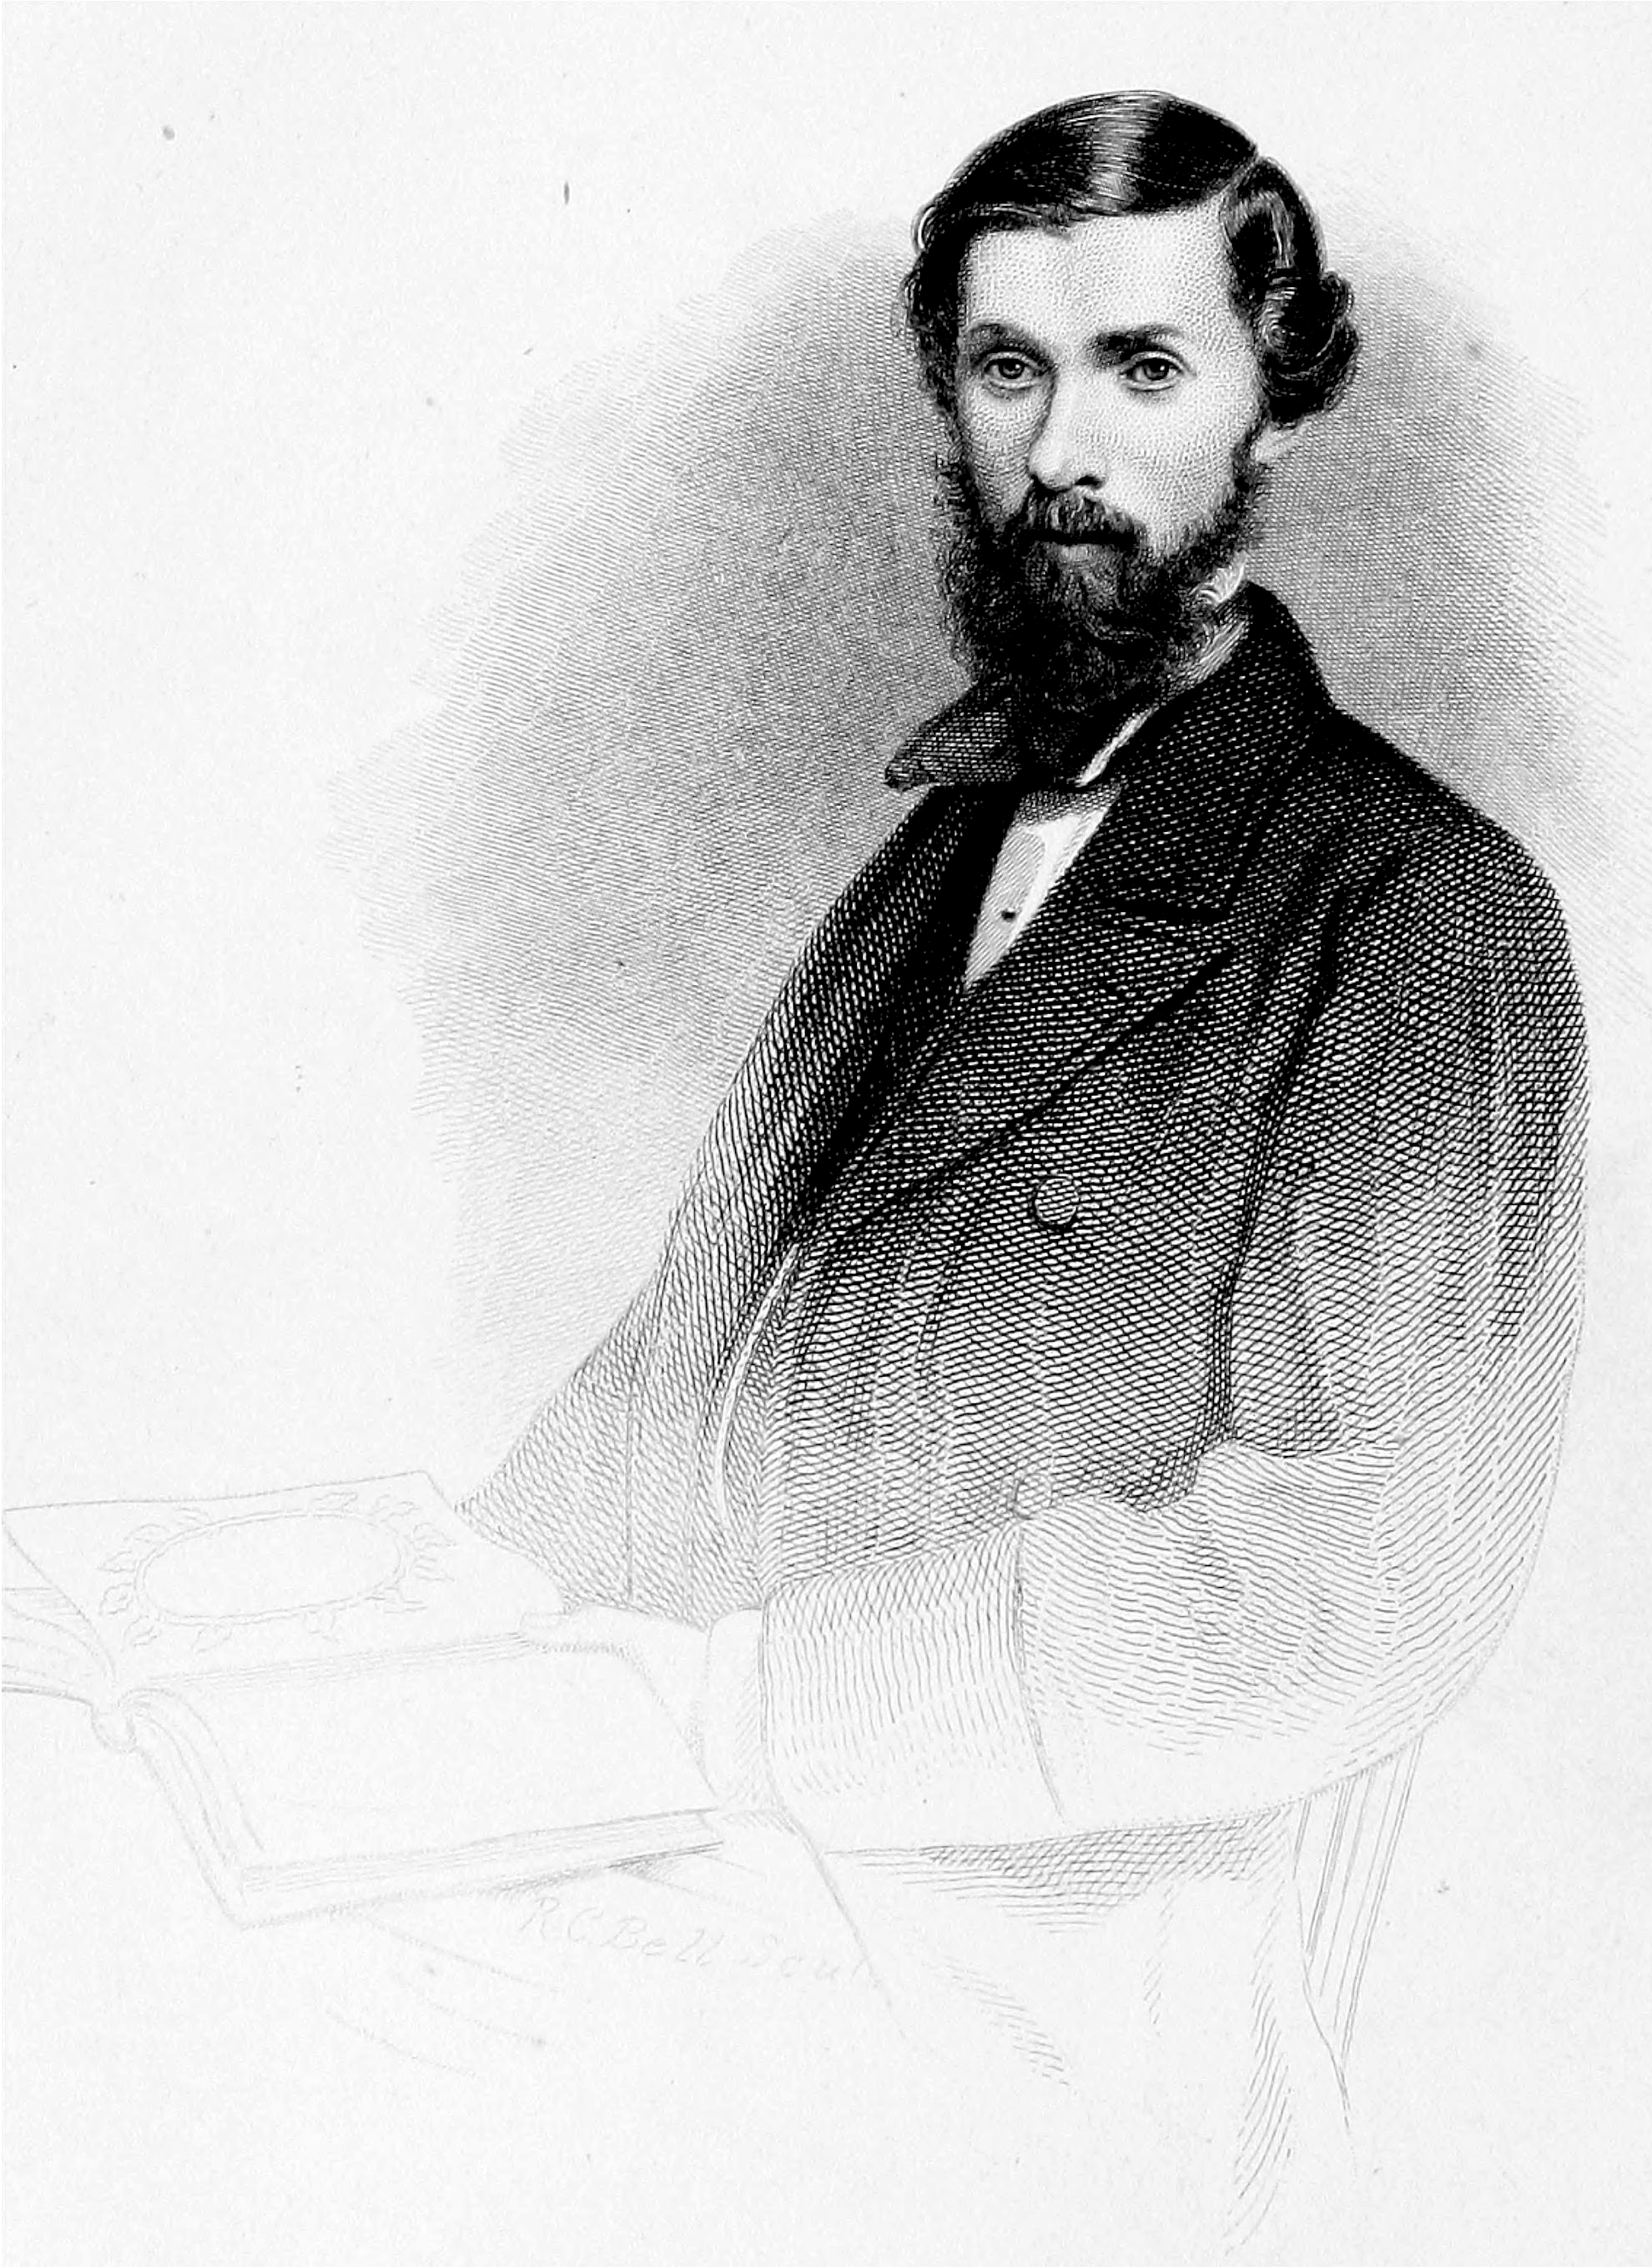
\includegraphics[width=0.7\linewidth]{Figure/R/Frontispiece_to_Memoir_of_the_late_Alexander_Henry_Rhind,_of_Sibster}
\end{figure}
\lemma{relazione}
\lemma{retta}Per Euclide\pointsto~\seeentry{Euclide}\index{Euclide} ente geometrico fondamentale insieme a punto e piano.
\llemma{r. complanari}Rette che appartengono allo stesso piano.
\llemma{r. incidenti}Rette complanari che hanno un punto in comune.
\llemma{r. parallele}Rette complanari che non hanno un punto in comune.
\llemma{r. perpendicolari}
Se due rette sono incidenti e formano quattro angoli retti le rette sono perpendicolari.
\llemma{r. sghembe}Rette non complanari che non hanno punti in comune.
% !TeX encoding = UTF-8
% !TeX spellcheck = it_IT
% !TeX root = MatDiz.tex
\chapter{S}
\vspace{5mm} 
\lemma{segmento}Parte di una retta compresa tra due punti distinti della retta.\llemma{s. adiacente}Due segmenti sono adiacenti se appartengono alla stessa retta.\llemma{s. consecutivo}Due segmenti sono consecutivi se hanno un vertice\pointsto~\seeentry{vertice} in comune.
\lemma{semiperimetro}La metà del perimetro\pointsto~\seeentry{perimetro}. Viene indicato con il simbolo $P$.
\entry{semipiano}Ciascuna delle due parti in cui viene divisa un piano\pointsto~\seeentry{piano} da una retta.
\entry{semiretta}Ciascuna delle due parti in cui viene divisa una retta\pointsto~\seeentry{retta} da un punto.
\lemma{seno}L'origine del termine è la seguente. In sanscrito il termine per indicare seno era \textit{jya-ardha} semi corda, abbreviato in \textit{jya}. Gli arabi tradussero questo termine in \textit{jiba}. Tale parola era scritta \textit{jyb}. I primi traduttori latini scambiarono questo vocabolo con \textit{jaib} che significa baia e tradussero tale parola con \textit{sinus} che ha analogo significato \cite{Gheverghese2000}.\titolettoa{Definizione} dato un triangolo rettangolo\pointsto~\vedilemma{t. rettangolo} definiamo seno dell'angolo il rapporto tra il cateto\pointsto~\vedilemma{cateto} opposto\pointsto~\vedilemma{o. lato} all'angolo e l'ipotenusa\pointsto~\vedilemma{ipotenusa} $\sin\beta=\frac{\text{opposto}}{\text{ipotenusa}}$. \titolettoa{Definizione} data una circonferenza goniometrica\pointsto~\vedilemma{c. goniometrica} diremo seno l'ordinata\pointsto~\vedilemma{ordinata} del punto di intersezione tra il raggio\pointsto~\vedilemma{raggio} e la circonferenza \vref{fig:sdefinizioneseno}.
\titolettoa{Definizione} data una circonferenza il seno è la meta di una corda\pointsto~\vedilemma{corda} che unisce due punti distinti sulla circonferenza. \llemma{f. seno}
\begin{figure}
	\scaptionb{Funzione seno grafico}
	\label{fig:sfunzioneSeno}
	\includestandalone[width=0.8\linewidth]{Figure/senografico}
\end{figure}
La funzione seno\pointsto~\vedilemma{goniometria} è definita in $\R$  a valore in  $[-1,1]$. La funzione  è limitata\pointsto~\vedilemma{f. limitata}.
La funzione è periodica\pointsto~\seeentry{f. periodica}  di periodo $k\pi\quad k\in\Z$. La figura~\vref{fig:sfunzioneSeno} rappresenta il grafico della funzione.
\begin{figure}
	\scaptionb{Seno definizione}
	\label{fig:sdefinizioneseno}
	\includestandalone[width=\linewidth]{Figure/senodefinizione}
\end{figure}
\lemma{SI}Sistema Internazionale delle unità di misura.
\lemma{sistema di riferimento}sistema che permette di individuare la posizione di un punto.\llemma{s. di riferimento cartesiano} 
\lemma{sessagesimale}Sistema di numerazione a base sessanta. Di origine babilonese viene usato per il calcolo del tempo e nella misura degli angoli.
\entry{somma}Risultato dell'addizione\pointsto~\seeentry{addizione}.
% !TeX encoding = UTF-8
% !TeX spellcheck = it_IT
% !TeX root = MatDiz.tex
\chapter{T}
\vspace{5mm} 
\lemma{tangente}
\lemma{triangolo}Poligono  piano con tre lati. Gli estremi di un triangolo si chiamano vertici.\llemma{t. perimetro} Il perimetro\pointsto~\seeentry{perimetro} del triangolo di lati $a$, $b$, $c$ è $2P=a+b+c$.\llemma{t. area} L'area del triangolo è $A=\frac{\text{base}\cdot \text{altezza}}{2}$\pointsto~\seeentry{base}\pointsto~\seeentry{altezza}. \llemma{t. rettangolo}
% !TeX encoding = UTF-8
% !TeX spellcheck = it_IT
% !TeX root = MatDiz.tex
\chapter{U}
\vspace{5mm} 
\lemma{uguaglianza} Il simbolo di uguaglianza $=$ venne introdotto da Robert  Recorde \pointsto~\seeentry{Recorde Robert}\index{Recorde Robert} nel 1557\cite{Kline1972}
% !TeX encoding = UTF-8
% !TeX spellcheck = it_IT
% !TeX root = MatDiz.tex
\chapter{V}
\vspace{5mm}
\lemma{vertice}Punto di intersezione lati di un poligono. Punto in comune ai lati di una angolo\pointsto~\vedilemma{angolo}.%
\entry[Viete Francois]{Viète François} François\index{Viète Fraçois}(1540-1603) Studiò legge . Fu consigliere privato di Enrico di Navarra. Fu un matematico per hobby introdusse le lettere per rappresentare le incognite e le costanti.\cite{Kline1972} \cite{Boyer1980}
% !TeX encoding = UTF-8
% !TeX spellcheck = it_IT
% !TeX root = MatDiz.tex
\chapter{W}
\vspace{5mm} 
\lemma{Widmann}Johannes (1460 - 1505)\index{Widmann Johannes}, introdusse per la prima volta, i simboli più $+$ e meno $-$ nel libro \foreignlanguage{german}{\textit{Mercantile Arithmetic or Behende und hüpsche Rechenung auff allen Kauffmanschafft}} pubblicato a Lipsia nel 1482.
% !TeX encoding = UTF-8
% !TeX spellcheck = it_IT
% !TeX root = MatDiz.tex
\chapter{X}
\vspace{5mm}
% !TeX encoding = UTF-8
% !TeX spellcheck = it_IT
% !TeX root = MatDiz.tex
\chapter{Y}
\vspace{5mm}
% !TeX encoding = UTF-8
% !TeX spellcheck = it_IT
% !TeX root = MatDiz.tex
\chapter{Z}
\vspace{5mm}
\lemma{zero}Elemento neutro dell'addizione\pointsto~\vedilemma{addizione}.
\llemma{z. funzione}
Data una funzione\pointsto~\vedilemma{funzione} $\funzione{f}{A}{B}\;a\in A$ è uno zero per la funzione se $f(a)=0$
%------------------------
%\include{appendice}
\backmatter
%include{abbordi}

\pagestyle{plain}
\twocolumn
%\onecolumn

\printbibliography
\clearpage
\printindex
\clearpage
\listoftables
\clearpage
\listoffigures
\cleardoublepage[empty]
%\include{colophon}
\end{document}
